\documentclass[smallcondensed]{svjour3}

\usepackage{dblfloatfix}
\usepackage{url}
\usepackage{color}
\usepackage{varwidth}
\usepackage{graphicx}
\usepackage{quoting}
\quotingsetup{vskip=4pt,leftmargin=10pt,rightmargin=8pt}
%\usepackage{csquotes}
\graphicspath{{./imgs/}{../jpeg/}}
\DeclareGraphicsExtensions{.pdf}
\usepackage{tabularx,booktabs,rotating,multirow,multicol}
\usepackage[noadjust]{cite}
\usepackage{caption}
\usepackage{color}
\usepackage[roman]{parnotes}
\usepackage[many]{tcolorbox}
\usepackage[symbol,para]{footmisc}
\usepackage[strings]{underscore}
\usepackage{tikz,dcolumn,booktabs,lscape}% <- sparklines chart embedded in tables
\usetikzlibrary{positioning}

\newif\ifdraft
\drafttrue

\makeatletter
\renewenvironment{quotation}
               {\list{}{\listparindent=0pt
                        \itemindent    \listparindent
                        \leftmargin=8pt
                        \rightmargin=10pt
                        \topsep=4pt
                        \parsep        \z@ \@plus\p@}
                \item\relax\itshape``}
               {\relax``\endlist}
\makeatother

\setlength{\rotFPtop}{0pt plus 1fil}% <- add this line after loading rotating
\setlength{\rotFPbot}{0pt plus 1fil}% <- maybe its better to add this line too

%\renewcommand\thesubsubsectiondis{}
%\newcommand{\Subsubsection}[1]{\subsubsection{\underline{#1}}}
%\newcommand{\Subsubsection}[1]{\subsubsection{#1}}
\hyphenation{op-tical net-works semi-conduc-tor}
% This will go in the next version of parnotes.sty
\makeatletter
\def\parnoteclear{%
    \gdef\PN@text{}%
    \parnotereset
}
\makeatother

% Plot a tiny Likert bar chart
% Input:
%   #1 Coordinate data
%   #2 Mean value
%   #3 Array of values
\newcommand{\likertplot}[3]{%
    \begin{tikzpicture}[xscale=0.25, yscale=0.015, baseline]
        \begin{scope}[ycomb, yscale=0.3]
            \draw[ultra thin, black!20] (1,#2)--(5,#2);
            \draw[black!80, line width=2mm] plot #1;
%            \foreach [count=\i] \x in {#3}
%            {
%              \draw[shift={(\i,0)}] 
%                (0pt,3pt) -- (0pt,-3pt) node[below,font=\scriptsize] {$\x$};
%            }
        \end{scope}
    \end{tikzpicture}%
}

\newcommand{\likertscale}[1]{%
    \begin{tikzpicture}[xscale=0.25, yscale=0.01, baseline={(0,-0.3)}]
        \begin{scope}[ycomb, yscale=0.4]
            \foreach [count=\i] \x in {#1}
            {
              \draw[shift={(\i,0)}] 
                (0pt,3pt) -- (0pt,-3pt) node[below,font=\small] {$\x$};
            }
        \end{scope}
    \end{tikzpicture}%
}

\def\boldif#1{\ifdraft\textbf{**#1**\newline\indent}\else\relax\fi}

\def\checkmark{\tikz\fill[scale=0.33](0,.35) -- (.25,0) -- (1,.7) -- (.25,.15) -- cycle;}

\newcolumntype{L}{>{\hsize=.8\hsize\raggedright\arraybackslash}X}
\newcolumntype{R}{>{\raggedleft\arraybackslash}X}
\newcolumntype{C}{>{\centering\arraybackslash}X}
\newcommand\setrow[1]{\gdef\rowmac{#1}#1\ignorespaces}
\newcommand\clearrow{\global\let\rowmac\relax}
\clearrow

%\newcommand\comment[1]{}
%\newcommand{\comment}[1]{{\noindent\bfseries #1\\}}
%\newcommand\todo[1]{{\noindent\color{red}\\\textbf{TODO:~}#1\\}}
%\newcommand\todo[1]{}

\begin{document}
\title{Processes, Barriers, and Resolution Strategies for Merge Conflicts}

\author{Nicholas Nelson \and Caius Brindescu \and Shane~McKee \and Anita Sarma \and Danny Dig}

\institute{Nicholas Nelson \and Caius Brindescu \and Shane McKee \and Anita Sarma \and Danny Dig
\at Oregon State University, Corvallis, OR 97331\\\email{\{nelsonni,brindescu,anita.sarma,digd\}@oregonstate.edu, mckeesh@outlook.com}
}

\maketitle

\begin{abstract}
Merge conflicts occur when developers make concurrent changes to the same part of the code.
They are an inevitable and painful aspect of collaborative software development.
Because of that tool builders and researchers have focused on the prevention and automatic resolution of merge conflicts.
However, there is little empirical knowledge about how developers actually approach and perform merge conflict resolutions.
Without such knowledge, tool builders might be building on the wrong assumptions and researchers might miss opportunities for improving the state of the art.

We conducted semi-structured interviews of 10 software developers across 7 organizations, including both open-source and commercial projects.
We identify key processes, techniques and perceptions from developers, which we extend and validate via a two surveys, of 102 developers and 162 developers.

We find that developers are directly impacted by their perception of the complexity of the conflicting code, and may alter the timeline in which to resolve these conflicts, as well as the methods employed for conflict resolution based upon that initial perception.
Developers' perceptions alter the impact of tools and processes that have been designed to preemptively and efficiently resolve merge conflicts.
Understanding whether developers will react according to standard use cases is important when creating human-oriented tools to support development processes.
\end{abstract}

%!TEX root = main.tex

\section{Introduction}\label{introduction}

Collaborative development is essential for the success of large projects~\cite{hattori2010syde}, and is enabled by version control systems. 
In Git, and other version control systems, developers work on their changes in isolation; periodically synchronizing them by merging with the main line of development. 
This can be problematic, because developers can concurrently change the same code, without being aware of each others' changes.
These overlapping changes become evident when they try to merge their work into the main line, and encounter a \emph{merge conflict.}
In the majority of cases, the merges succeed.
However, research has shown~\cite{cassandra,Brun2011} that in open source projects, merge conflicts occur in approximately 19\% of all merges.

Resolving merge conflicts is nontrivial, especially when the changes diverge significantly~\cite{Brun2011}.
The resolution process can be tedious and can cause delays as developers figure out how to approach and resolve conflicts~\cite{cassandra}. 
Poorly-performed merge conflict resolutions have been known to cause integration errors~\cite{bird-branches-conflict}, workflow disruptions, and jeopardize project efficiency and introduce delays~\cite{estler2014awareness}. 

Developers are aware of the problems posed by merge conflict resolutions.
They follow different informal processes to avoid encountering, or having to resolve conflicts; e.g. sending out emails to the rest of the team, performing partial commits, or racing to finish changes~\cite{deSouza2003breaking,cataldo2008distributed_dev}.
Unfortunately, these practices come with their own problems, and can make the resolution of a merge conflict even harder~\cite{Brun2011}. 

Past work examined different mechanisms for proactive merge conflict detection~\cite{Brun2011,palantir,Guimaraes}, proposed tools for resolving merge conflicts~\cite{nishimura,mens2002state}, and discussed advantages of syntax- and semantic-aware merge tools~\cite{danny_refactorings,hunt2002extensible,apel_semistructured_2011}. 
However, several key questions remain unanswered: 
How do developers approach and manage merge conflicts?
How do developers perceive the difficulty of a merge conflict resolution? 
Do the current tools support developers' merge conflict resolution needs?
Without such knowledge, tool builders might be building on wrong assumptions and researchers might miss opportunities for improving the state of the art.

To answer these questions, we talked directly to developers.
This is crucial to understanding problems in the context in which they occur~\cite{fritz2010using, sillito2006questions, ko2007information}.
We interviewed 10 software developers from 7 organizations about their experiences and perceptions of merge conflicts. % in the software development process.
Our participants had a median of 5 years of software development experience, and work on a mix of both small-scale (less than 10 contributors) and large-scale projects (greater than 1000 contributors).
These interviews helped us understand how developers approach and manage merge conflicts, and their unmet needs within their processes and tools.

To triangulate our findings and provide a broader understanding of developers' processes, techniques, tools, barriers, and perceptions of merge conflicts, we deployed two surveys to a larger population of software developers.
We use two surveys to split the topics into manageable lengths and reduce fatigue on participants.
The surveys sampled 102 and 162 developers (264 developers in total).
For both surveys, the majority of our participants had 6 or more years of software development experience, and reported facing merge conflicts a few times a week.

To understand the effects and implications of software developers' processes and strategies, we answer the following research questions:

\begin{itemize}[label=$\bullet$]
\item \textbf{RQ1:} How do software developers manage merge conflicts?
\subitem \textbf{RQ1a:} How do software developers become \textbf{aware} of merge conflicts?
\subitem \textbf{RQ1b:} How do software developers \textbf{plan} for merge conflict resolutions?
\subitem \textbf{RQ1c:} How do software developers \textbf{evaluate} merge conflict resolutions?
\item \textbf{RQ2:} What difficulties do software developers experience when managing merge conflicts?
\item \textbf{RQ3:} How well do tools support developer's needs for managing merge conflicts?
\end{itemize}

We found that developers, when initially assessing a merge conflict, rely on the \textit{code complexity of the conflicting lines} and \textit{their own knowledge in the area of the conflict} as the top two factors when estimating the difficulty of a merge conflict resolution.
These concerns cause developers to alter their resolution strategy, and in some cases delay the resolution, which can have negative consequences.

After understanding the merge conflict, developers must resolve the conflict in order to return to normal development.
We found that the key challenges that developers face when resolving conflicts are \textit{understanding the conflicting code,} and having enough meta information about the conflicting code (who made the change, why, and when).
Developers rely heavily on \textit{their knowledge of the conflicting code} when implementing their merge resolutions.

Our findings show that developers perceive that an \textit{increase in conflict complexity} has a greater impact on the resolution difficulty, than an increase in the size of the conflict.
However, development tools lack features that address this dimension.
This could partially be alleviated by focusing on the tool improvements most desired by developers: \textit{better usability, better information filtering,} and \textit{better history exploration.}

%In the context of these findings, we present implications for researchers, tool builders, and practitioners.
%For example, researchers have previously developed merge conflict avoidance and resolution tools that need to be simplified and brought into alignment with the basic merging tools used by software practitioners.
%Tool builders should create merging tools that provide more context-sensitive information about conflicting code, and do so when scaling to more complex merge conflicts.

Overall, we make the following contributions.
\begin{enumerate}
\item We introduce a model of developers' processes for managing merge conflicts, from the point of awareness to the resolution of a conflict;
\item We discuss proactive and reactive strategies developers use when monitoring for merge conflicts;
\item We provide evidence for the prevalence of deferring a merge conflict resolution, and the knock-on effects of doing so;
\item We provide empirically-derived rankings of factors that developers perceive as increasing the difficulty of a merge conflict resolution;
\item We expose disparities between developers' needs when resolving merge conflicts, and the features provided by development toolsets.
%\item We present actionable implications that researchers, tool builders, and practitioners can build upon.
\end{enumerate}

This article extends the work presented at ICSME in 2017~\cite{mckee2017software}: 
(1) by providing a model of developer's processes for managing merge conflicts; 
(2) conducting an additional \emph{Processes Survey} for validating our model and examining developers' strategies, and; 
(3) extending the \emph{Barriers Survey} results by further analysis based on our model. 
%!TEX root = main.tex

\section{Related Work}\label{related_work}

\subsection{Collaboration}

Gousios et al. \cite{integrator_perspective} conduct a study in which they ask integrators to describe difficulties in maintaining their projects and code contributions. 
They showed that integrators have problems with their tools, have trouble with non-atomic changesets, and rank \textit{git knowledge} in the top 30\% of their list of biggest challenges. 
Gousios et al.~\cite{gousios2016work} additionally conducted a study into the challenges of the pull-based model from the perspective of contributors. 
They found that most challenges relate to code contribution, the tools and model used to contribute, and the social aspects of contributing (specifically highlighting merge conflicts).
These works focus on the collaborative processes that go into contributing to open-source projects and operating as integrators within them, whereas we examine the processes and issues inherent to merge conflicts and the tools built to support their resolution.

Guzzi et al.~\cite{Guzzi2015} conducted an exploratory investigation and tool evaluation for supporting collaboration in teamwork within the IDE.
They found that developers working within a variety of companies were able to quickly and easily resolve merge conflicts, and did this using merge tools.
However, they also note that although automatic merging was used, their participants also manually checked each conflict and suggest that this reveals some mistrust of tools.
Guzzi et al. further explain that their interviewees avoid merge conflicts by using strict policies and software modularity.
Their results complement our findings that toolset mistrust is a major concern, and that standards need to be implemented in order to avoid complex merge conflicts.

Begole et al.~\cite{begole_work_2002} investigate the work rhythms of developers.
They use minute-by-minute records of computer activity coupled with locality of the activity, calendar appointments, and e-mail activities to provide meaningful visualizations for group coordination.
The passive nature of developers' interaction with these visualizations requires users to engage and coordinate with each other, which differs from version control systems that actively support the software development process.

These works highlight the importance of collaboration and coordination in the daily activities of developers, which provide impetus for our examination of developers adaptations in the presence of merge conflicts, which represents a breakdown in those activities.

\subsection{History Understanding and Navigation}

Codoban et al.~\cite{Mihai_lenses} seek to evaluate developer understanding and usage of code history. 
Our results show that tool support during history exploration factors a moderate amount into the difficulty of a merge conflict (N10). 
This result independently verifies their findings that developers experience tool limitations in usability (I1) and history visualization (I4).

Ragavan et al.~\cite{ragavan_pfis-v_2017} propose an Information Foraging Theory (IFT) model for how developers forage in the presences of history (in their paper they refer to this as ``variations'').
This model highlights the needs of developers attempting to understand variations in code, whereas we examine the methods and strategies that developers employ prior to encountering a merge conflict and the processes for evaluating their resolutions.

While these studies provide an insight into how developers use, explore, and understand history, they do not approach any of the problems that collaboration can bring to software development.
We aim to examine the complete process from awareness of a merge conflict to it's eventual resolution.

\subsection{Better Merge Conflict Resolution}

Currently, all version control systems treat source code files as text.
Therefore, merging is done at a textual level, ignoring all structure that the files might contain.
Several researchers have looked at ways to improve this status quo.

Westfechtel~\cite{westfechtel_structure-oriented_1991} propose a merging technique that uses the structural (i.e. lexical) information of a language when performing a merge. However, such tools are language dependent and the required algorithms are expensive to run.
Apel et al.~\cite{apel_structured_2012-1, apel_semistructured_2011} propose \emph{JDime}, which improves existing structured merging techniques by only using structural information when the unstructured (i.e. text only) merge has failed.
Binkley et al.~\cite{binkley_program_1995} propose using call graph information to correctly merge different versions of the program.

Lippe and van Oosterom~\cite{lippe_operation-based_1992} go a different way.
They propose a new merging technique, \emph{operation-based merging} that would replay the changes that were performed on the two branches, in the order in which they were performed.
Dig et al.~\cite{danny2008tse} uses this technique and shows empirically that many more merge conflicts could be solved by a tool that understood the semantics of change operations.

These studies seek to improve the performance and reliability of merging tools, which complement our results which show that toolset mistrust is a major concern among developers.
By addressing the quality and consistency of the algorithms and tools available for merge conflicts, tool builders can hopefully improve developer trust in the future.

\subsection{Workspace Awareness} 

Biehl et al.~\cite{biehl_fastdash:_2007} propose \emph{FastDASH}, a tool that fosters awareness between members of a team. 
FastDASH provides a dashboard that shows the files that are checked out, modified, and staged by other members of the team.
da Silva et al.~\cite{da_silva_lighthouse:_2006} propose \emph{Lighthouse} to show the changes being made at the design level.
Their tools presents all changes from the perspective of changes to the model (in the form of UML diagrams) of all of the developers project.
While all these approaches provide awareness of potential conflicts, they require the developer to actively monitor and discern if a conflict is likely or has occurred.

Sarma et al.~\cite{palantir, sarma_palantir:_2003} go a step further and propose \emph{Palant\'{i}r}.
Palant\'{i}r monitors other developer's workspaces, and, depending on the changes, will notify the developer, in a non-obtrusive manner, if a conflict has happened.
Similarly, Hatori and Lanza~\cite{hattori2010syde} propose \emph{Syde} that monitors the changes at an Abstract Syntax Tree (AST) level.
This allows the tool to give more precise information to the developer.

Brun et al.~\cite{Brun2011} propose \emph{Crystal}, which monitors selected branches in the repository. 
Crystal preemptively merges the branches in the background and will notify the developers of any conflicts that arise. 
It detects both \emph{direct} conflicts (changes to the same line), and \emph{indirect} conflicts (changes to a different line that cause build or test failures).
Guimara\~{e}s et al.~\cite{Guimaraes} propose \emph{WeCode}, which also merges in uncommitted code, in order to improve the time to detection of a merge conflict.

Servant et al.~\cite{servant_casi:_2010} proposes \emph{CASI}, that uses visualization to help developers detect conflict early.
CASI shows all the program elements that are influenced by the changes made in the team, so that developers can coordinate more efficiently.

Kasi and Sarma~\cite{kasi_cassandra:_2013} take a more proactive approach and propose a novel task scheduling approach that aims to minize the number of conflicts. 
\emph{Cassandra} uses developer preferences, task and file dependencies to schedule tasks so that they are less likely to conflict.

%!TEX root = main.tex

\section{Methodology}\label{methodology}

%We employed exploratory interviews with software practitioners and surveys of practitioners to validate our findings.

To understand the merge conflict processes, barriers, and resolution strategies of software developers, we used mixed methods consisting of interviews to gather qualitative insights, and surveys to provide quantitative triangulations into the broader context of merge conflicts.
Mixed methods allow us to identify perspectives and themes from both individual and population-wide samples to strengthen the validity of both, as per guidelines from Easterbrook et al.~\cite{easterbrook2008selecting}.

We conducted \textit{Exploratory Interviews} with software developers to create a taxonomy of processes, barriers, strategies, and concerns experienced by developers when encountering and resolving merge conflicts.
We then triangulate and extend the results of our interviews by conducting a \textit{Processes Survey}~(S1) and a \textit{Barriers Survey}~(S2) using concepts and vocabulary generated from the interviews. 

Processes are developed to address common problems in teams and organizations.
Identifying the problems developers face is an essential element for process improvements~\cite{beecham2003software}.
We conducted a \textit{Processes Survey}~(S1) of software developers to understand how they monitor for merge conflicts, how they plan their resolution strategies, and their processes for evaluating whether their resolutions are successful.

To analyze the scale of barriers, constraints, and concerns of software developers when approaching merge conflicts, we conducted a separate \textit{Barriers Survey}~(S2) of software developers.
In this survey, we sought to extend the results from our interviews and to include additional questions relating to tools, technology, and coordination within development teams.

\subsection{Exploratory Interviews}\label{interviews}

Semi-structured interviews provide qualitative data collection through open-ended questions that elicit interviewee's thoughts and opinions about a particular topic.
The resulting data includes themes and terminology from the perspective of the interviewee, as opposed to the interviewer, and provides a context for further quantitative inquiry~\cite{easterbrook2008selecting}.

We conducted semi-structured interviews with software developers to understand their concerns when facing merge conflicts and the factors that impact merge conflict difficulty.
We selected interview participants from top contributors to open-source projects, and from industry contacts using snowball sampling~\cite{goodman1961snowball} to reach a larger sample size.
Finally, we asked each participant to identify additional practitioners for recruitment to our study.

We interviewed ten software developers from seven different organizations spanning six different industries.
Eight of the participants worked primarily on open-source projects.
Participants worked on a variety of project sizes; from projects with less than five active contributors, to more than 1700 contributors (as evaluated by analyzing code repositories for a 12-month period).
Table~\ref{interview_demographics} provides additional demographics data, including software development experience, role, industry, project size, and whether the participant primarily focused on open- or closed-source software development.
Each interview lasted between 30 to 60 minutes.
Participants were offered US\$50 in either cash, gift card, or a donation to a charity of their choice.

\begin{table}[!htbp]
\renewcommand{\arraystretch}{1.3}
\caption{Interview Participant Demographics}
\label{interview_demographics}
\centering
\begin{tabularx}{\textwidth}{@{}llllrr@{}}
\toprule
	\parnoteclear % tabularx will otherwise add each note thrice
	\textbf{Par.}\parnote{Par. = Interview participant} & \textbf{Exp.}\parnote{Exp. = Years of software development experience} & \textbf{Role} & \textbf{Industry} & \textbf{Source}\parnote{Source = Source code licensing in primary project} & \textbf{\mbox{Contrib.}}\parnote{Contrib. = Approximate number of individual contributors in primary project (between March 2016-March 2017)\vspace*{-0.3\baselineskip}}\\
\midrule
	P1 & 18 yrs. & Sr. \mbox{Software} \mbox{Developer} & Semiconductor Mfr. & Open & 1700\\
	P2 & 6 yrs. & Software \mbox{Engineer} & Semiconductor Mfr. & Open & 1700\\
	P3 & 3 yrs. & Software \mbox{Engineer} & Semiconductor Mfr. & Open & 1700\\
	P4 & 10 yrs. & Software \mbox{Developer} & Academia & Open & \textless10\\
	P5 & 3 yrs. & Infrastructure \mbox{Engineer} & Healthcare Software & Closed & \textless10\\
	P6 & 5 yrs. & Software \mbox{Developer} & Healthcare Software & Closed & \textless10\\
	P7 & 5 yrs. & Software \mbox{Engineer} & Business Software & Open & 200\\
	P8 & 25 yrs. & Director & Academia & Open & 600\\
	P9 & 8 yrs. & Software \mbox{Developer} & IT Services & Open & 600\\
	P10 & 2 yrs. & Software \mbox{Developer} & Sports Software & Open & \textless5\\
\bottomrule
\end{tabularx}
\parnotes
\end{table}

At the beginning of the interview we gave participants a short explanation of the research goals, our definition of merge conflicts, and collected demographics data. 
We then asked participants about the roles that they play in their project, their experience working in team settings, questions about merge conflicts, the process of conflict resolution, and the difficulties that they faced in conflict resolution.

We formulated the interview questions about merge conflicts in order to understand how developers perceived and how they approached merge conflicts.
The following is an example of some of the questions we asked in the interview.
The full set of questions can be found in our companion site~\cite{companion_site}.
\begin{itemize}
	\item Can you describe a merge conflict, or a set of conflicts, that you would consider to be the typical case?
	\item Do you have any particularly memorable merge conflict resolutions that you can recall?
	\item Have you had some code structures, design patterns, coding styles, etc., that you would consider a ``usual suspect'' in a conflict?
	\item What kind of measures would you take to minimize the amount of defects that you introduce?
\end{itemize}

The semi-structured interview format allowed participants to provide us with unanticipated information~\cite{seaman2008qualitative}. 
Further, we allowed open-ended discussion about merge conflicts in general at the end of the interview, which allowed participants to share ideas and topics that they found particularly important. 
We continued interviewing participants until we reached saturation in the answers, which was measured using topic saturation as our benchmark~\cite{fusch2015we}.

\subsection{Processes Survey (S1)}\label{processes_survey}

Merge conflicts disrupt the collaborative development workflow, and developers have adapted and developed different processes for handling these complexities.
To understand the common structure and prevalence of these processes we use surveys, which are used for mapping the state of practice, establishing baselines for investigating research topics, and gathering opinions regarding software engineering technologies and practices~\cite{deMello2016survey}.
Therefore, we conducted a 15-question \textit{Processes Survey} (S1) of software developers that included both open-ended and predefined questions.

We recruited participants from contributor lists on popular open-source repositories on GitHub, advertised on social networking sites (Twitter and Reddit), and by directly contacting software developers via email.
Due to the nature of social media and mailing lists, we cannot compute a response rate from these distribution methods.
We observe that 35.29\% of participants were located outside of the United States and several participants indicated that they sent the survey onward to other software developers.

The survey was conducted online and anonymity was guaranteed.
The \textit{Processes Survey}~(S1) was available for 38 days and we received 113 survey responses, however, 11 responses were incomplete, resulting in 102 total responses.
The results of this survey are presented in Section~\ref{results}.

\begin{figure}[!htbp]
\centering
\hspace*{-0.7cm}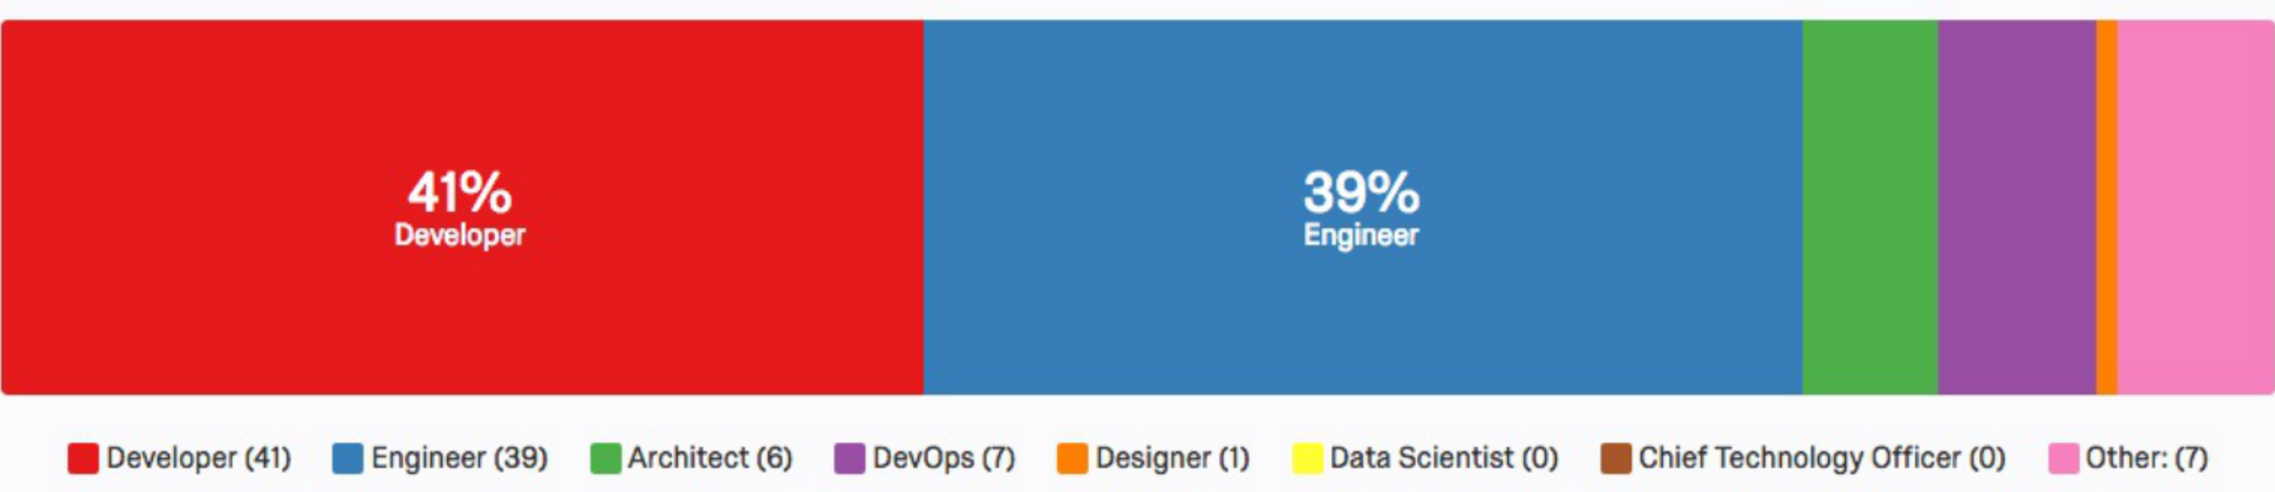
\includegraphics[width=1.105\textwidth,keepaspectratio]{ProcessesParticipantRoles}
\caption{Distribution of primary roles from Processes Survey~(S1) participants: 45.5\% are primarily a \textit{Developer}, 42.0\% an \textit{Engineer}, 12.5\% \textit{Other}, and 12.8\% were either \textit{DevOps}, \textit{Architect}, or \textit{Designer}. No participants selected \textit{Data Scientist} or \textit{Chief Technology Officer}.\vspace*{-0.3\baselineskip}}
\label{processes_roles}
\end{figure}

Survey participants had a mean of 9.1 years of programming experience, and primarily worked in teams of 2-5 members (45.10\% overall).
Participants were assumed to be software developers in some capacity, but primary roles within individual organizations can differ throughout the industry.
Participants were given seven different roles to select, as well as an \textit{Other} field to provide additional roles not included in the pre-populated options.
Figure~\ref{processes_roles} provides a visual illustration of the distribution of primary roles among participants.
87.5\% of participants were primarily a \textit{Developer} or \textit{Engineer} (45.5\% and 42.0\% respectively), with 6.9\% selecting \textit{DevOps}, 5.0\% \textit{Architect}, 1.0\% \textit{Designer}, and 12.5\% \textit{Other}.
Among participants that selected \textit{Other}, the open-text responses included: ``Tester,'' ``Security Analyst,'' ``Hobbyist Programmer,'' and ``Researcher.''

We divided the survey into four categories, with each containing 3-5 questions (see \cite{companion_site} for individual questions).
First, we elicited background information about demographics, roles, and experience.
Second, we asked questions relating to how and when developers become aware of merge conflicts.
Third, we asked questions related to planning and implementing merge conflict resolution strategies.
Finally, we asked questions about evaluating the effectiveness of those merge conflict resolutions and the particular tools that are used throughout the processes of working with merge conflicts.

\subsection{Barriers Survey (S2)}\label{perceptions_survey}

In the last step, we conducted a 50-question \textit{Barriers Survey} of software developers in order to examine the barriers, constraints, and concerns experienced when encountering merge conflicts.
We developed questions to confirm, extend, and broaden the results from the interviews.

\renewcommand*{\thefootnote}{\arabic{footnote}}
%\setcounter{footnote}{0}
We recruited participants for \textit{Barriers Survey}~(S2) to be similar to \textit{Processes Survey}~(S1) participants so that we could compare and triangulate the results.
We therefore recruited participants from contributor lists on popular open-source repositories on GitHub, advertised on social networking sites (Facebook, Twitter and Reddit), and by directly contacting software developers via email. 
Participants spanned a variety of organization structures and geographical locations, giving generalizability to results.
The survey was conducted online and anonymity was guaranteed in order to elicit honest responses from participants.
The \textit{Barriers Survey}~(S2) was available for 56 days and we received 162 survey responses, but individual parts of the survey have varying response rates and are reported where appropriate in Section~\ref{results}.

Survey participants were given six different software roles to select, and in many cases, participants considered themselves to be fulfilling multiple roles. 
Table~\ref{survey_roles} provides a pairwise breakdown of participants' role selections, with a majority of participants considering themselves to be \textit{Software Engineer/Developer} (95.1\% overall).
Survey participants indicated a median software development experience of 6-10 years (36.4\% overall), and worked on project sizes ranging from 2 to more than 51 developers (the median was 2-5 developers, constituting 48.8\% of all responses).

\vspace*{-0.8\baselineskip}

\begin{table}[!htbp]
\caption{Barriers Survey (S2) Participant Roles\textsuperscript{i}}
\label{survey_roles}
\centering
\begin{tabularx}{\textwidth}{@{}r|*{10}{C}c@{}}
\toprule
\addlinespace[4.5em]
	& \begin{rotate}{30} Soft. Developers \end{rotate} 
	& \begin{rotate}{30} Sys. Architects \end{rotate} 
	& \begin{rotate}{30} DevOps \end{rotate} 
	& \begin{rotate}{30} Project Managers \end{rotate}
	& \begin{rotate}{30} Project Maintainers \end{rotate}
	& \begin{rotate}{30} Sys. Admins \end{rotate}
	& \begin{rotate}{30} Other \end{rotate}\\
\midrule
	Software Developers & 154 & & & & & & \\
	System Architects & 53 & 54 & & & & & \\
	DevOps & 51 & 34 & 53 & & & & \\
	Project Managers & 44 & 29 & 20 & 44 & & & \\
	Project Maintainers & 39 & 21 & 24 & 22 & 40 & & \\
	Systems Administrators & 22 & 16 & 15 & 14 & 12 & 23 & \\
	Other & 8 & 4 & 4 & 3 & 1 & 2 & 11 \\
\bottomrule
	\multicolumn{8}{c}{\noindent\parbox[t]{11.7cm}{\vspace{0.4em}\textsuperscript{i}\hspace{0.2em}\textit{Barriers Survey}~(S2) participants were allowed to select multiple roles. Each entry represents the number of participants that selected both of the roles indicated for the column and row. 62 out of 162 participants (38\%) selected three or more roles.}\vspace*{-0.3\baselineskip}}
\end{tabularx}
\end{table}

We divided the \textit{Barriers Survey}~(S2) into four categories, each category containing 5-7 questions (see \cite{companion_site} for a list of questions).
First, we elicited background information about demographics, roles, and experience.
Second, we asked questions related to difficulties that developers experience when encountering merge conflicts.
Third, we asked questions related to conflict resolution and the factors that affect developers.
Finally we asked questions about the tools and tool features that developers use when working with merge conflicts.
Questions were presented either as 5-point Likert-type scales (with no pre-selected answers) or open-ended text forms to gather additional insights.

\subsection{Data Analysis}\label{analysis}
To ensure that our survey samples are representative of the larger developer population, we compare the demographics from the \textit{Processes Survey}~(S1) and the \textit{Barriers Survey}~(S2) with the results of the 2018 StackOverflow Developer Survey\footnote{https://insights.stackoverflow.com/survey/2018}.

The 2018 StackOverflow Developer Survey was conducted on 101,592 software developers from 183 countries.
This survey includes the number of years spent coding professionally by 77,903 participants.
%, and is presented as totals for buckets of 0-2 years, 3-5 years, 6-8 years, 9-11 years, 12-14 years, 15-17 years, 18-20 years, 21-23 years, 24-26 years, 27-29 years, and 30 or more years.
%For comparison purposes, we similarly grouped the results from the \textit{Processes Survey}~(S1) and the \textit{Barriers Survey}~(S2).
Figure~\ref{populations} provides a graphical representation of the percentile distribution of professional programming experience among participants in the \textit{Processes Survey}~(S1), \textit{Barriers Survey}~(S2), and the 2018 StackOverflow Developer Survey.
We see that our sample population has more experienced developers, and the trends match between all three samples.

\begin{figure}[!htbp]
\centering
\fbox{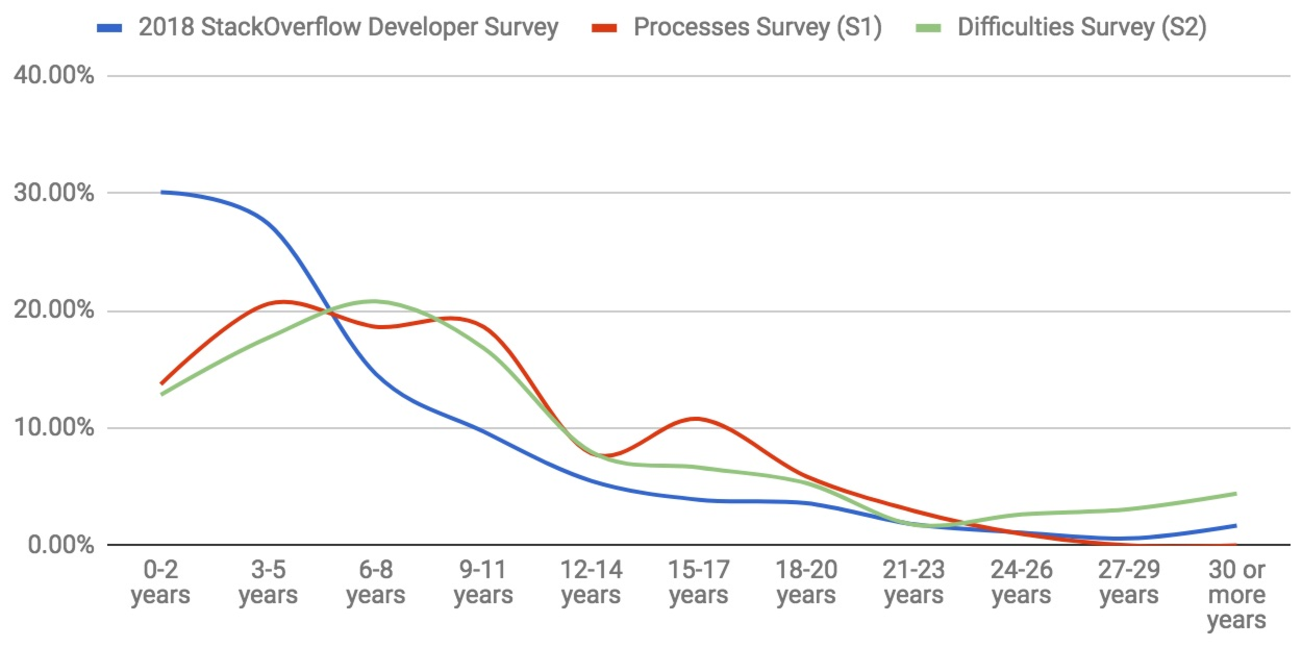
\includegraphics[width=0.98\textwidth,keepaspectratio]{imgs/populations}}
\caption{Percentile distributions of professional programming experience compared between \textit{Processes Survey}~(S1), \textit{Barriers Survey}~(S2), and 2018 StackOverflow Developer Survey participants. Responses are inclusively binned into 3-year buckets for comparison across surveys.\vspace*{-0.3\baselineskip}}
\label{populations}
\end{figure}

To further compare the distribution of programming experience across these population samples, we conduct nonparametric tests of the equality of the probability distributions between two samples.
Comparing \textit{Processes Survey}~(S1) responses with 2018 StackOverflow Developer Survey responses, we conclude that we cannot reject the null hypothesis that these samples were drawn from the same population distribution (Two-sample Kolmogorov-Smirnov test, $D = 0.33636$, p-value$ = 0.5939$).
We similarly conclude that \textit{Barriers Survey}~(S2) responses and 2018 StackOverflow Developer Survey responses could plausibly be drawn from the same population distribution (Two-sample Kolmogorov-Smirnov test, $D = 0.27273$, p-value$ = 0.8326$).
In both cases, we cannot reject the null hypothesis that the survey sample population is the same as the 2018 StackOverflow Developer Survey population, therefore, we conclude that our samples are representative of the development community.

\subsubsection{Interview Analysis}

Interviews were audio-taped and transcribed. 
The first and third authors unitized~\cite{unitization} the interview transcripts into cards that each contained a single logically consistent statement. 
To organize these cards we employed card sorting, a collaborative technique of exploring how people think about a certain topic~\cite{spencer2009card,card_sort}, which allows key concepts and associations to be identified through an open sorting method that iteratively develops categories during the process.

We performed two iterations of the open card sorting process.
In the first iteration, we developed a standardized coding scheme and improved it to an acceptable point through \textit{negotiated agreement,} which was reached when no further thematic categories could be created and agreed upon by both coders~\cite{garrison2006revisiting,ritchie2013qualitative}.
The coding scheme dictated that sentences must be consecutive and topically related to be grouped into a single card.
Logically connected statements that were separated by other lines were considered to be separate cards, as a conservative measure to preserve context within each card.

In the second iteration, the first and third authors sorted cards according to our coding scheme and discussed the resulting taxonomies until consensus was reached.
Based upon our research questions, we grouped the resulting categories as follows: the processes that developers use for merge conflicts (Section~\ref{RQ1}, the difficulties that developers face with merge conflicts (Section~\ref{RQ2}), and the impact of development tools on the resolution process (Section~\ref{RQ3}).

\subsubsection{Survey Analysis}

For the \textit{Processes Survey}~(S1), we evaluated the distribution of survey answers for each of the four Likert-type question by analyzing across demographic categories.
We used Likert-type questions to measure the extent to which participants agreed with a particular statement, or the degree to which a factor has impacted the participant.
Where answers differed across a demographic category, we note the difference and provide further discussion of these results.

The \textit{Processes Survey}~(S1) contained five open-ended questions.
We performed open thematic coding~\cite{fereday2006demonstrating} to analyze the responses to these questions.
The resulting codebook, including descriptions and examples, are available on our companion site~\cite{companion_site}.
%Table~\ref{tab:codes} provides the resulting codebook, including descriptions and examples.
After establishing a codebook, the first two authors independently coded the responses to each open-ended question.
For question 7 (\textit{``How do you monitor for merge conflicts?''}), we achieve an inter-rater reliability (IRR) agreement of $0.95$ (Jaccard similarity coefficient).
For questions 8 (\textit{``How do you determine the urgency of a merge conflict?''}), 11 (\textit{``What is your first step in trying to understand code involved in a merge conflict?''}), 14 (\textit{``What effect did deferring your response to a merge conflict have on the resolution of the conflict?''}), and 19 (\textit{``If your first attempt at resolving a merge conflict fails, what backup strategies do you use?''}), we achieve IRR agreements of $0.81$, $0.88$, $0.74$, and $0.92$, respectively (all are above the Software Engineering research standard of $0.80$ IRR).

%\def\shift{\hspace{0.5em}}
%\begin{table}[!htbp]
%\centering
%\caption{Codebook used for coding open-ended responses from Processes Survey (S1)}
%\label{tab:codes}
%\begin{tabular}{lp{1.5in}p{1.3in}}
%\toprule
%Code & Description & Example \\
%\midrule
%\multicolumn{3}{l}{\textbf{Q7: How do you monitor for merge conflicts?}} \\
%\shift Proactive & & \\
%\shift Reactive & & \\
%\midrule
%\multicolumn{3}{l}{\textbf{Q8: How do you determine the urgency of a merge conflict?}} \\
%\shift Project Structure & & \\
%\shift Code Under Conflict & & \\
%\shift External Dependencies & & \\
%\shift No System & & \\
%\midrule
%\multicolumn{3}{p{4.5in}}{\raggedright\textbf{Q11: What is your first step in trying to understand code involved in a merge conflict?}} \\
%\shift About the conflict & & \\
%\shift The Code Itself & & \\
%\shift Analyzing the code & & \\
%\shift Design Concerns & & \\
%\shift Project Organization & & \\
%\shift No-op & & \\
%\midrule
%\multicolumn{3}{p{4.5in}}{\raggedright\textbf{Q14: What effect did deferring your response to a merge conflict have on the resolution of the conflict?}} \\
%\shift Physical Manifestations & & \\
%\shift External to company impact & & \\
%\shift Policy/culture changes & & \\
%\shift The Nuclear Option & & \\
%\shift Increased Complexity & & \\
%\shift Stop the presses & & \\
%\shift No-op & & \\
%\midrule
%\multicolumn{3}{p{4.5in}}{\raggedright\textbf{Q19: If your first attempt at resolving a merge conflict fails, what backup strategies do you use?}} \\
%\shift Collaborating & & \\
%\shift Redoing changes & & \\
%\shift Take it offline & & \\
%\shift Try again & & \\
%\shift No strategy/Other & & \\
%\bottomrule
%\end{tabular}	
%\end{table}

We evaluated the results of the \textit{Barriers Survey}~(S2) by performing open card sorting on the all open-ended questions.
The resulting categories were standardized to an acceptable point through \textit{negotiated agreement}~\cite{ritchie2013qualitative}.

The \textit{Barriers Survey}~(S2) was primarily composed of Likert-type questions, which were used to measure the extent to which participants agreed with a particular statement.
This means that lower mean and median values indicate less agreement with the statement in a particular question.
We use this design to validate both the degree of agreement to the interview results, as well as the existence of individual factors.

We present the results of the \textit{Exploratory Interviews,} \textit{Processes Survey}~(S1) and \textit{Barriers Survey}~(S2) in Section~\ref{results}.
When necessary, we refer to individual survey participants by a combination of the survey short-hand (S1 or S2) and participant number; for example S1--14 is participant 14 from the \textit{Processes Survey}~(S1) responses.
\section{Results}\label{results}

\boldif{Results from interviews indicated that a common model of operating with merge conflicts exists.}
To understand how developers manage merge conflicts, we asked interview participants to describe their current processes for handling merge conflicts.

\boldif{\textit{Add anecdotal quotes and descriptions from interviews to highlight these observations.}}
Participants talked about different steps that they follow, including using tools that alert them to potential or current merge conflicts, processes for analyzing and understanding conflicting code prior to implementing a resolution, and the use of tools for validating that their resolution worked.
As an example, P3 said:
\begin{quoting}
\textit{``Part of my job on the integration team requires that I check for bad regressions. I use scripts to track patches as they're being backported, so I know when and where to look if [a patch] introduces a conflict. [\ldots] And once I've fixed [the conflict], I try to compare with the previous version to make sure [the code] works in a similar way.''}
\end{quoting}

\boldif{Provide descriptions that link the stages of Merge Conflict model to this quote. Use it to drive description of simplified model description paragraph}

\boldif{Based on these anecdotal observations, we construct an initial model of the processes that developers employ when working with merge conflicts, see Fig.~\ref{model}.}
Our interview and survey results suggest that developers follow a series of phases through which they manage the life-cycle of individual merge conflicts.
We construct a model of the developer processes for managing merge conflicts and examine each phase in detail.
Figure~\ref{model} provides an illustration of this model. 
It consists of four phases: \emph{awareness, planning, resolution,} and \emph{evaluation.}

\boldif{Discuss the fact that no other studies have shown that a model exists for merge conflicts}

\begin{figure}[!htbp]
\centering
\fbox{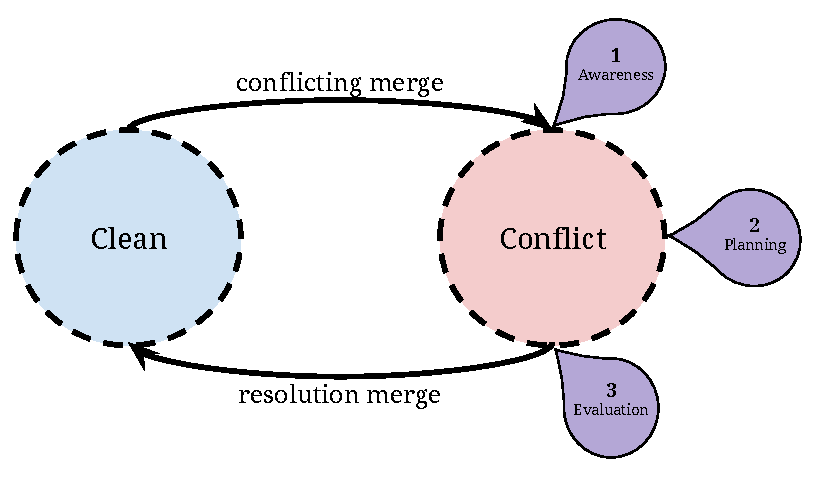
\includegraphics[width=0.90\textwidth,keepaspectratio]{imgs/MergeConflictModel}}
\caption{Model of Developer Processes for Managing Merge Conflicts. Developers alternate between \textit{clean} and \textit{conflicting} states of code. Beginning from (1)~\textit{development}, developers maintain (2)~\textit{awareness} of conflicts within the codebase in different ways. Once aware, developers begin (3)~\textit{planning} for a (4)~\textit{resolution} to fix the conflict. And finally, developers (5)~\textit{evaluate} the effectiveness of their deployed resolutions (returning to \emph{planning} if the resolution failed).\vspace*{-0.3\baselineskip}}
\label{model}
\end{figure}

\boldif{Awareness is how developers become aware}
First, the \emph{awareness} phase consists of the actions developers take to become aware of merge conflicts.
This could be passive, as the developer will become aware of a merge conflict when attempting to merge changes or perform a pull.
At the other end of the spectrum are developers who \emph{proactively} monitor for merge conflicts as they write code.
They are actively looking for changes that might be problematic, either manually or through the use of specialized tools.

\boldif{Planning is when developers plan their future actions}
Second, the \emph{planning} phase occurs after the developer has become aware that a conflict has occurred, and they are about to tackle the conflict.
This includes the decision of when they will try and resolve the conflict.
Some developers might try and resolve it immediately, while others might postpone the resolution.
Some might change their strategy depending on the conflict, incoming deadlines, or availability of resources.
This also includes other actions, such as if they are going to tackle the conflict alone, or collaborate with other developers knowledgeable in the area of conflict~\cite{CostaSarma}.

\boldif{Resolution is the action of implementing a resolution. Mundane and well understood, so we focus on the other three.}
Third, the \emph{resolution} phase represents the implementation of the planned resolution.
Several tools exist that help in this phase~\cite{nishimura,mens2002state,Brun2011}.
Here we focus on the difficulties that developers face during these resolution implementations (see Section~\ref{RQ2}).

\boldif{Evaluation is how developers check that their solution is correct}
Finally, after the conflict has been resolved, developers enter in the \emph{evaluation} phase.
In this phase, the developer has to evaluate their resolution before considering the conflict as resolved.
This is to ensure the correctness of the resulting code.
Possible actions during this stage includes compiling the source code.
Developers wanting more guarantees can go a step further and run the tests.
Finally, some groups have policies such as code reviews that need to be performed on the merge conflict resolution.
 
\boldif{To explore and validate this model, we asked developers to reflect upon how they become aware of merge conflicts, how they plan for merge conflict resolutions, and how they evaluate their resolutions in the \textit{Processes Survey}.}
In order to explore and validate this model, and our assumptions, we conducted the \emph{Processes Survey}.
Our aim in this survey was to understand how developers become aware of merge conflicts (what steps they take, what tools they use, etc.).
Also, we wanted to investigate their strategies for dealing with merge conflicts and how they decide whether the resolution has addressed all of their concerns.

Results are categorized according to the life-cycle of merge conflicts; with specific results for the \textit{awareness} (Section~\ref{RQ1}), \textit{planning} (Section~\ref{RQ2}), and \textit{evaluation} phases (Section~\ref{RQ3}).
We then present the difficulties that developers experience when managing merge conflicts (Section~\ref{RQ4}).
And finally, we examine the gaps in tool support for managing merge conflicts according to developer's needs (Section~\ref{RQ5}).
%!TEX root = main.tex

\section{Discussion}\label{discussion}

\subsection{Awareness Phase}

\boldif{Developers do not regularly actively monitor for merge conflicts. ...}
The results presented in Section~\ref{RQ1a} show that only a third of developers actively monitor for merge conflicts.
When developers are caught unaware of the conflict, they are more likely to be interrupted by it.
This can lead to more frustrations, the they do not have any warning of when the conflict will occur.

\boldif{Therefore their approaches are mostly \emph{reactive,} and their tool selection reflects that.}
When we looked at the processes developers employ we found that most developers employ \emph{reactive} processes, even if they \emph{proactively} monitor for a merge conflict.
This can be seen as a problem of the tools that developers have at their disposal.
All the tools mentioned support only a \emph{reactive approach,} which biases developers towards one particular solution.
If developers want a more proactive approach, they need to come up with their own solution.
The most options is to increase communication.
While this technique might be effective in large teams, it scales very poorly, and cannot be effectively used in larger organizations. 

\boldif{All the above point towards a need for better collaborative tools, that promote a proactive approach}
Our results point to the conclusion that developers are not aware of existing proactive tools (e.g. Palant\'{i}r~\cite{sarma_palantir:_2003}, Crystal~\cite{Brun2011}).
Furthermore they are note leveraging the advantages these tool bring to the table. %TODO Add at least one advantage here.

\subsection{Planning phase}

\boldif{25\% of developers consider all conflicts as being equally urgent.}
One quarter of all developers consider all merge conflicts to be equally urgent.
We can assume that most developers will interrupt their work regardless of the type of merge conflict.
Therefore, they will give the same level of attention, for example, to a conflict generated by whitespace, or formatting changes, as a conflict that is generating by conflicting logical changes. 

\boldif{The research community needs to pay attention to developers needs when it comes to categorizing MC.}
Even if the developers use a \emph{reactive} monitoring approach to detecting merge conflicts, better tool support can make their lives easier.
For example, instead of notify a developer that a merge conflict has occurred, adding an annotation as to the type of conflict might help developers.
This will give them enough information to know how urgent the merge conflict really is, without having to interrupt their workflow.

\boldif{60\% of developers defer a merge conflict, at least once. However, there doesn't seem to be a systematic understanding of the effect of such a deferral.}
The responses indicate that 60\% of developers have deferred a merge conflict at least once. 
Developers have listed multiple reasons for deferral, however two stand out: complexity and the number of conflicting regions.
Both these indicate that a developer will defer if the conflict resolution looks lengthy, either because the changes are not trivial, or simply because there are a lot of smaller conflict to solve.

\boldif{The results of such a deferral can be disastrous. However, it is difficult to make an assessment of the effect of the deferral when the decision to defer is being made.} 
The results of deferring can be disastrous. 
Participants reported having to throw away code (the \emph{Nuclear Option}) and even having customer or users noticing broken functionality.
However, it is difficult to make an assessment of when a deferral can turn a merge conflict into an even bigger problems.
Tools could provide such information, in order to help developers make accurate and informed decisions to prevent issues further down the line.

\boldif{Some developers do not have an approach for dealing with merge conflicts.}
Finally, an interesting result is that some developers do not have a strategy for approaching a merge conflict resolution.
The existence of this \textit{no strategy} approach is anecdotal, but curious, since we assume that developers are rational actors seeking to organize themselves in ways that increase the likelihood of successful outcomes.
And yet this strategy appears to go counter to that notion.
On of the explanations for the lack of a strategy is the lack of experience, as they did not encounter enough situations to form a strategy.
\subsection{Resolution phase}

\boldif{@Nick: This requires some discussion from S2 - ICSME paper.} %TODO discussion about resolution strategies from S2/interviews.

\subsection{Evaluation phase}

\boldif{Tests are still the most common criteria for determining a merge conflict resolution successful.}
The 2 most common criteria that developers mentioned is that the \emph{code compiles,} and that \emph{all tests pass.}
However, less then half selected both options.
While tests passing can be considered a good criteria, the fact that the code compiles is not.
Even if the code compiler, there might be logical errors that are introduced during the merge resolution process, especially if the merge conflict resolution was a difficult one.

\boldif{Only a minority of developers mention that code review is part of their success criteria}
Interestingly, only a minority of developers mentioned code review as part of their success criteria (37.25\%).
%TODO add citation for the code review part
While code reviews are an effective way to detect bugs introduced in the code base, the practice does not seem to be applied to code changed during merge conflict resolution.

\boldif{Some developers have only a myopic view of a correct resolution, relying on eyeballing it and basic compilation}
Many developers replied that they use an informal approach for validating the results of a merge conflict resolution.
A majority (64.7\%) of the respondents mentioned that one of their criteria is that the merge result \emph{``looks good.''}
Experience can play a big factor, as this method is highly subjective.

\boldif{Some approaches will only detect direct merge conflicts, not indirect ones.}

\boldif{There is a lack of tool support that makes it difficult for developers to properly evaluate the success of a merge conflict resolution.}

\boldif{Failed merge conflict resolution are a somewhat common occurrence. Backup strategies vary.}
Finally, almost large majority of our respondents have mentioned that they have had failed merge conflict resolutions.
The most common backup strategies, are in a way, opposite.
They either take the merge conflicts ``offline,'' and work on them without impacting others in the team, or they will choose to bring another pair of eyes to the table, and collaborate with someone in order to resolve the conflict.

\boldif{Some strategies reveal that developers find it easier to reimplement, than to figure out what went wrong.}
The two most intriguing strategies are developers \emph{trying again,} and \emph{redoing the changes.}
\emph{Trying again} implies that developers think that they might have missed something, and that by going through the changes again, they might catch or have a better understanding of the two changes that are conflicting.
On the other hand, the fact that 14 developers mention that they \emph{redo the changes} shows that the \emph{Nuclear Option} is more used that we initially observed.
This option is very expensive, as developers have to redo their changes, from scratch on top of what can possibly be new code.
Tools should provide better merging support, so developers can resolve a conflict and not have to scrap good code just because it happens to intersect with other changes.


\section{Implications}\label{implications}

\subsection{For Developers}
Developers are in the middle of any situation involving merge conflicts, and the efforts required to resolve them.
Understanding the constraints that different phases of the merge conflict life-cycle place on time and resources can allow more effective prevention and management of any merge conflicts that do arise.

Developers indicate that understanding code, having appropriate information, and dealing with complex codesets are key themes of difficulty when working with merge conflicts (Sections~\ref{RQ1}, \ref{RQ2}).
Existing tool support can help with some of these issues, but developers also need to educate themselves on development processes that prevent and alleviate the severity of merge conflicts. 
For example, the number of conflicting files and the size of changes are considered important factors (Section~\ref{difficulty-factors}).
Researchers~\cite{brindescu2014versioncontrol} have previously found that developers using distributed version control systems commit more often, and that committing more often makes debugging easier when something breaks~\cite{meyer2014continuous}.
Therefore, developers should strive to make smaller commits, and commit often.

Other agile development processes such as continuous integration, iterative development, and branch merging policies are known to facilitate development in large, distributed teams. 
However, not all developers are actively using such techniques~\cite{phillips2011branching}, and large organizations will require additional diligence in order to address the increased possibility of conflicts occurring.
These organizations should strive to use proactive merge conflict monitoring and detection systems and processes, to speed up the transition from the \textit{awareness} and \textit{planning} phases and on through to the \textit{resolution} and \textit{evaluation} phases.

\subsection{For Tool Builders}
Version control systems provide an easy method for storing and retrieving recent development history, but examining older development history at scale and in a usable manner has not completely met developers' expectations.
Tool builders should work to address this unmet need by leveraging research in search systems for developer-assistance~\cite{nabi2016putting} and machine learning-based code assistance~\cite{bradley2011history_exploration} to provide intuitive and expressive tools for history exploration.

Even if developers use a \emph{reactive} monitoring approach for detecting merge conflicts, better tool support can make their lives easier.
For example, instead of notifying a developer that a merge conflict has occurred, adding an annotation within tools indicating the type of conflict might assist developers.
This type of contextualized information would allow developers to more precisely know how urgent the merge conflict is, without having to interrupt their workflow.

Developers indicate that current merge toolsets do not scale to handle large, complex merge conflicts (see Section~\ref{tool_effectiveness}).
To address this concern, tool builders should look at consolidating feature sets that currently span multiple tools in order to provide better usability (I1 from Table~\ref{s2_tool_improvements}).
Tool builders should also add more expressive search and filtering features for both project history and meta-information related to merge conflicts (I2, I3), to ease the frustration of developers that must understand the context and evolution of code involved in the conflict.

Before starting a merge conflict resolution, we found developers having to ``guess-timate'' the difficulty of the conflict resolution to decide whether to work on it now or deffer it, whether to integrate the changes or simply start over. 
Prediction tools that identify the complexity of conflicts and difficulty of resolution can help alleviate this.
This will provide to developers with enough information to make accurate and informed decisions in order to prevent further issues down the line.

When it comes to evaluating the result of a merge conflict resolution, we found that developers employ various strategies (Table~\ref{conditionsSuccess}).
Developers mentioned that passing tests (C1) and successful compilation (C2) are some of the criteria for success.
However, for large projects, running the test suite can be time intensive.
Tools can help developers by providing information or running only tests that are impacted by the conflict resolution.
This would help developers as they would have to rely less on their own intuition (C5), when it comes to evaluating the result.

\boldif{Conflicts might be difficult, because the result is hard to evaluate}
The fact that developers mention code complexity as one of the main factors in deferring a merge conflict resolution, and that developers ``eyeball'' the resolutions, seems to be an indication that evaluation might be a problem in the resolution.
Merge conflicts are perceived as difficult because \emph{the evaluation of the results are difficult.}
In this case, tools should provide better support for developers when they evaluate their resolution.

Finally, most developers have failed at least once in resolving a merge conflict resolution (Figure~\ref{fig:first-attempt-failure}).
Tools can provide better insight into why the resolution has failed, so developers have information to formulate their next steps.
Currently, when a merge conflict resolution fails, developers have to interrupt their workflow by taking the resolution offline (Table~\ref{backup-strategies}, B1), or they have to ask for help, which has the potential of interrupting other developers (B2).
If developers had more information about \emph{why} the merge conflict resolution failed, they might be able to recover more efficiently.

\subsection{For Researchers}
%Our results inform future research by providing insights into software developers' perspectives during merge conflicts.

The top factors that impact the assessment of merge conflict difficulty are primarily focused on program comprehension (F1, F3, F4 from Table~\ref{s2_factors}).
Program comprehension has been an important research focus, with entire conferences dedicated to it.
Previous research has explored tool support and visualizations to help comprehend programs, both small and large.
Our results indicate that developers still have unmet needs along the following dimensions: (1) comprehending code snippets in isolation, (2) understanding the code context underlying multiple code snippets that are split across multiple files, and commits, and; (3) the ability to quickly comprehend the complexity of these code snippets. 

%have a need to understand fragments of code, with some of this code split across multiples files, commits, or conflicting codebases.
%The ability to quickly evaluate the complexity of these code fragments is needed, including at the scale of text editors as evidenced by the use of basic toolsets instead of modern IDEs when working with merge conflicts (see Section~\ref{RQ3}).

Developers indicate that their needs during merge conflict resolutions center around the retrieval, organization, and presentation of relevant information (N1, N3, N4 from Table~\ref{s2_needs}).
With the variety of meta-information available across different toolsets, and the inconsistent use of terminology, there is a need for standardization and best practices to be developed.
Standardization efforts would likely help to alleviate some of the mistrust of merging tools that developers have expressed.
However, researchers should investigate the margin of errors that are tolerated by developers to determine the context in which developers discontinue use of tools.
 %threshold of merge tool errors that indicates whether a user will mistrust and discontinue use of those tools.

Expertise is seen as both a significant factor that affects the assessment of merge conflict difficulty (F2), and an important need for developers to effectively resolve the conflict (N2).
We have also seen that experience can play a part in developer's assessment of the success of a merge conflict resolution (C3).

Previous work has focused on recommending developers best suited to perform a collaborative merge based on the previous edits to conflicting files~\cite{dasilva2015niche} or developers' experience across branches and project history~\cite{CostaSarma}. 
However, these efforts have resulted in tools that require standalone installation and execution. 
Our results indicate that developers are concerned about toolset fragmentation, and therefore adding an additional tool might be counterproductive to the workflow of most developers. 

Our results show that 14 developers mention that they \emph{redo the changes} when a merge conflict resolution fails.
This \emph{Nuclear option} is very expensive.
Tools should provide better merging support, so developers can resolve a conflict and not have to scrap good code just because it happens to intersect with other changes.

Finally, we find that developers need to quickly estimate whether they can fix the conflict, and whether to resolve it now or delay the resolution. 
This indicates that developers need mechanisms to identify the skillsets required to complete the conflict resolution task, by viewing the code fragments (D1, D2).
Research should investigate mechanisms to identify required skillsets by using information retrieval or machine learning techniques on the code fragment and past edits.

\section{Threats to Validity}\label{threats}
As in any empirical study, there are threats to validity with our work.
We attempt to remove these threats where possible, and mitigate the effect when removal is not possible.

\paragraph{Construct Validity.}
Interview questions were open-ended and designed to elicit developer opinions about the experiences, difficulties, and perceptions of merge conflicts.
We determined particular factors and needs after concluding all interviews, and thus did not bias interview participants to only factors previously mentioned.
We created survey questions using factors found through card-based unitization.
This methodology allowed us to capture the common themes that developers experience when working with merge conflicts, but might have allowed themes specific to particular sub-groups to be unrepresented in our results.

\paragraph{Internal Validity.}
Confounding and extraneous factors can affect conclusions relating to cause and effect.
We lessen this effect by using multiple methods to triangulate our results, and compare against other datasets where appropriate.
Because we use these methods to highlight stronger answers, this also means that we may have missed subtle trends across our data that could have been visible otherwise.

\paragraph{External Validity.}
Interview results may not generalize to all developers due to a small sample size, but we reduce this effect by selecting interview participants from open- and closed-source projects, varying industries, and varying project sizes (see Table \ref{interview_demographics}).
To expand and confirm our interview results, we survey 102 and 162 developers on varying aspects to ensure our results match with trends in the larger software development community.
We do not report a response rate for our surveys, since social media and mailing lists do not allow accurate measurement of the number of individuals that read our recruitment message and did not choose to participate.


\section{Conclusion}\label{conclusion}
Practitioner perceptions of merge conflicts have an impact on their development process. First, they use perceptions to determine which tactics they will use to resolve the conflict.
After choosing how to resolve the conflict, practitioners encounter a new set of needs, both technical and social. 
Understanding these perceptions and needs is critical to understanding how to design tools which conform to the issues that these practitioners face in collaborative development.
We provide actionable implications for researchers, tool builders, and practitioners to harness the results of our study.
In future work, we hope to explore whether these factors, needs, and desired toolset improvements can be seamlessly merged into tools or techniques that assist developers' workflows.

%Merge conflicts interrupt development flow.
%Our work explores the human perceptions of merge conflict resolution in version control systems. We conducted an analysis of 10 interviews and confirmed our findings with a survey of 162 practitioners.
%
%We asked how practitioners approach merge conflicts and found that they identify 8 factors of importance for the initial evaluation of merge conflict difficulty. 
%We then asked which factors impact the difficulty of a merge conflict resolution and found 10 factors that impact the difficulty of the merge conflict resolution process. 
%These sets of factors serve as a way to inform managers and future research about merge-conflict-related difficulties of software practitioners.
%
%We also asked if developer tools met practitioner needs for merge conflict resolutions and found 6 improvements which practitioners would like to see in these tools. 
%In addition, we share specific tool needs from our interviews to give an idea of what people really struggle with in their merge conflict resolution workflows.
\section*{Acknowledgments}

We thank Iftekhar Ahmed, Amin Alipour, Alex Hoffer, Michael Hilton, Sruti Ragavan, and the anonymous reviewers for their valuable comments on earlier versions of this paper.
We also thank all of our interview and survey participants, especially those who helped distribute survey links.
This research was partially supported by NSF grants CCF-1439957, CCF-1553741, CCF-1560526, and IIS-1559657.


\bibliographystyle{spmpsci}
\bibliography{Bibliography,second}

\end{document}


